\chapter{Antennas}\label{ch:antennas}

With the requirements calculated in chapter \ref{ch:linkbudget}, it is now possible to design an antenna to overcome these requirements.  

\section{Dipole antennas}


\section{Reflector Antennas}

Reflector antennas are used places where a high gain and directivity is needed. The reflector antenna do also have a wide bandwith, which all together has made them poplar for deep space communication \citep{Imbriale2012}. Although reflector antennas can be made in different types, shapes and configurations, they all essentially consist of a passive reflecting surface illuminated by a smaller primary feed. The basic analysis is done using trigonometry which provides satisfactory result because the diameter of the reflecting surface often is ten times the wavelength. In figure \ref{fig:reflector_types} four main configurations is depicted. (a) is the on-focus parabolic reflector where the feed for the parabolic is placed F distance apart called the focal point. This would leave an area where the feed is placed, where there will be a gap in the coverage. This is omitted in (b) which is the off-axis reflector. This types has no gap in coverage and therefore is often used as radar. The (c) Cassegrain reflector and (d) Gregorian reflector uses both a feed in the middle of the reflector which then uses a second reflector at the focal point to reflect the energy back to the large reflector. Because of the large dimensions a reflector antenna are not suited for low frequencies < 2GHz. Using the equations \ref{eq:para1} to \ref{eq:para4} a design has been made for $f = 10GHz$, $\lambda = 30mm$, $D = 10\lambda = 300mm$, $\theta = 60^{\circ}$. This should give a gain at 30dBi. The design has been simulated in CST studio in figure \ref{fig:para_sim1} and \ref{fig:para_sim2}. The feeding antenna used is a dipole which is an omnidirectional antenna, this causes a loss in efficiency. An ideal reflector should be uniformly illuminated and all power should
be focused on the reflecting surface. The portion of the feed power that does not reach the reflector is referred to
as spillover loss while the ability to uniformly feed the parabola is referred to as illumination efficiency. Since
primary feeds have a tapered radiation pattern, a compromise between spillover losses and illumination
efficiency must be considered to maximize the aperture gain. In the simulation a gain at $G=15dB$ was obtained, this could be optimized using an horn-antenna. 

\begin{figure}[H]
\centering 
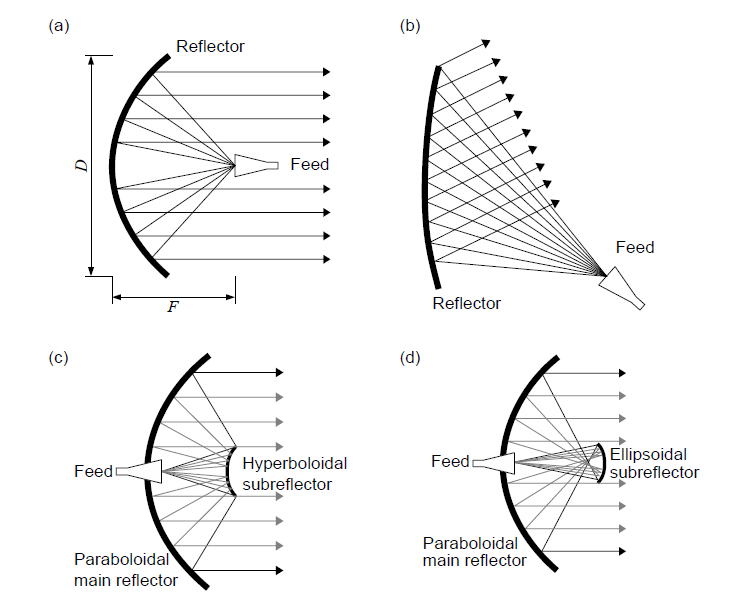
\includegraphics[scale = 0.7]{figures/antennas/reflector/types}
\caption{Reflector antenna configurations: (a) on-focus parabolic reflector; (b) off-axis reflector; (c) Cassegrain reflector; (d) Gregorian reflector \citep{Imbriale2012}}
\label{fig:reflector_types}
\end{figure}

Equation for parabola

\begin{equation}
y=a x^2 , a = \frac{1}{4F}
\end{equation}
\label{eq:para1}

Focal length
\begin{equation}
F=D\frac{1}{4tan(\theta/4)}
\end{equation}
\label{eq:para2}

Length of parabolic segment
\begin{equation}
L=\frac{ln(\sqrt{a^2 D^2 +1}+a D)}{4a}+\frac{D\sqrt{a^2 D^2 +1}}{4}
\end{equation}
\label{eq:para3}

Gain for parabolic reflector

\begin{equation}
G=\eta \frac{4\pi A}{\lambda^2}, A = \frac{\pi D^2}{4}
\end{equation}
\label{eq:para4}

\begin{figure}[H]
\centering 
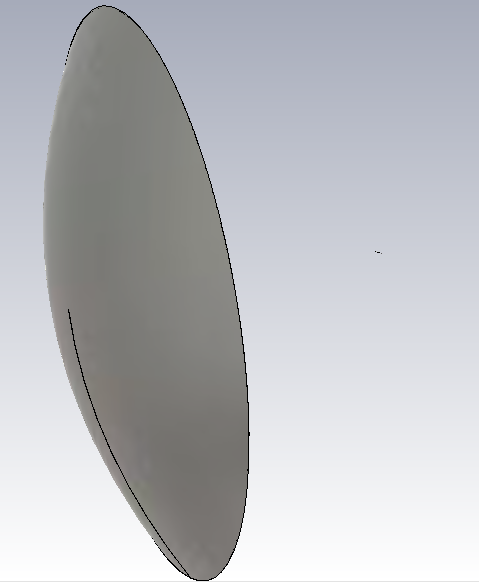
\includegraphics[scale = 0.5]{figures/antennas/reflector/parabola_cst}
\caption{Simulated reflector antenna in CST studio}
\label{fig:para_sim1}
\end{figure}

\begin{figure}[H]
\centering 
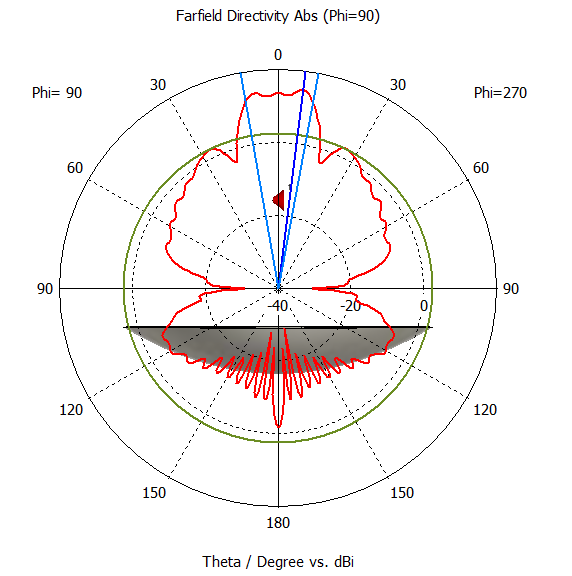
\includegraphics[scale = 0.5]{figures/antennas/reflector/parabola_cst_farfield}
\caption{Farfield of simulated reflector antenna in CST studio}
\label{fig:para_sim2}
\end{figure}



\section{Helical Antennas}

\subsection{Quadrifilar Helical Antenna}

\begin{figure}[H]
\centering 
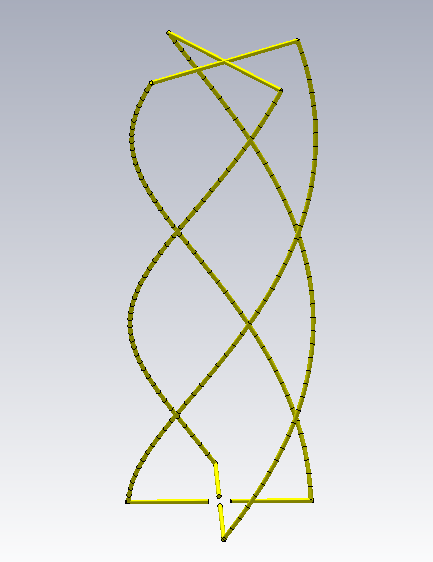
\includegraphics[scale = 0.7]{figures/antennas/qha/qha_6_1mhz}
\caption{QHA with $N=0.6$, $D=80mm$,$L=\frac{\lambda}{2}-D\cdot 0.75$, $f=1GHz$}
\label{fig:QHA1}
\end{figure}

The Quadrifilar Helical Antenna (QHA) (see figure \ref{fig:QHA1}) is an resonant antenna which is typically feed by two ports with a $90^\circ$ phase difference. The antenna has a circular polarization and the size is often smaller than a normal helical antenna. Typically the length of each arm is an integral multiple of the quarter-wavelength. The end of the helix
is open when the integer is odd, while short when the integer is
even \citep{Bai2014}. Despite the typically design the turn ratio, radius, length and feeding topology will affect the radiation pattern and polarization. Another important measure of all helical antennas is the pitch angle which is defined in equation \ref{eq:pitch}.

\begin{equation}
\alpha = tan^{-1}(\frac{S}{\pi D})
\end{equation}
\label{eq:pitch}

Where D is the diameter of the antenna, S is the spacing between the loops and futher N is the number of turns and L is the length of the antenna \citep{Balanis2005}.
\newline
\newline
An QHA has been build and simulated in CST studio. The dimensions are $D=80mm$,$L=\frac{\lambda}{2}-D\cdot 2$, $N=0.6$ at the frequency $f=122.5MHz$ and $\lambda = 2450mm$ with the wire diameter $Wd = 2mm$. The diameter is chosen so the antenna can be stowed in a 10x10x10cm box and the length is calculated so there is a half wavelength between the negative and positive side of a port. The feeding is done using two discrete ports as shoved in figure \ref{fig:QHA2}.  

\begin{figure}[H]
\centering 
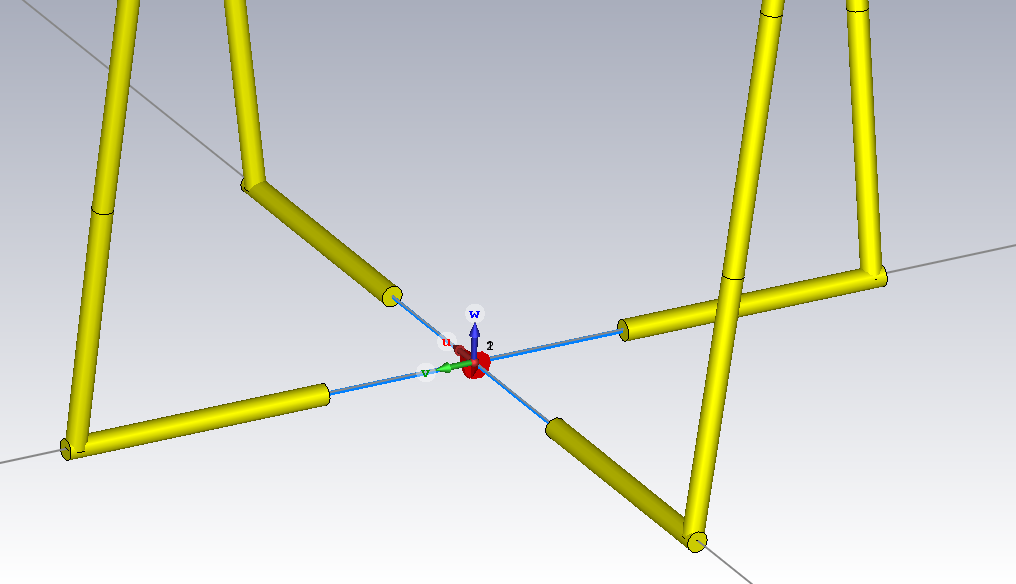
\includegraphics[scale = 0.4]{figures/antennas/qha/qha_6_feeding}
\caption{Feeding of the QHA for 122.5MHz using discrete ports}
\label{fig:QHA2}
\end{figure}
 
The QHA has been simulated and the results shows, that the antenna is matched to 131MHz even thou the S11 parameter at this frequency is only -2dB, see figure \ref{fig:QHA_S11}. The error is caused by the gap between the ports in the bottom and the extra length caused by the turn of N. It can be seen that the antenna also radiates at multiply of the match frequency and that the lowest return-loss is obtained at 4 times the frequency which gives 524MHz. The farfields for the frequencies 131,262 and 393MHz are shown in figure \ref{fig:QHA_ff_131}, \ref{fig:QHA_ff_262} and \ref{fig:QHA_ff_393}, where port 1 is fed with a positive phase at $90^\circ$. It is seen that the farfield not surprisingly changes with the frequency. The farfield suited best for tracking of ADS-B signals is the one in figure \ref{fig:QHA_ff_131}. \todo[inline,color=orange]{write someting about the earth curvature and why?}.      

\begin{figure}[H]
\centering 
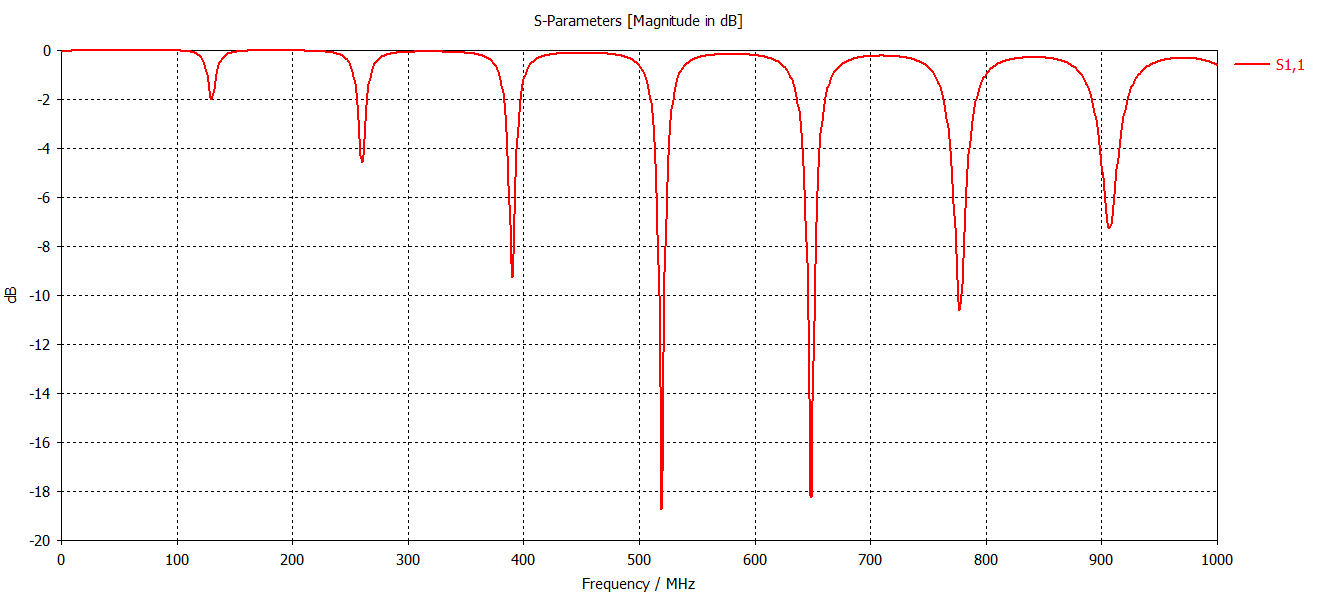
\includegraphics[scale = 0.5]{figures/antennas/qha/qha_6_S11}
\caption{S11 parameter of the QHA for 122.5MHz}
\label{fig:QHA_S11}
\end{figure}

\begin{figure}[H]
\centering 
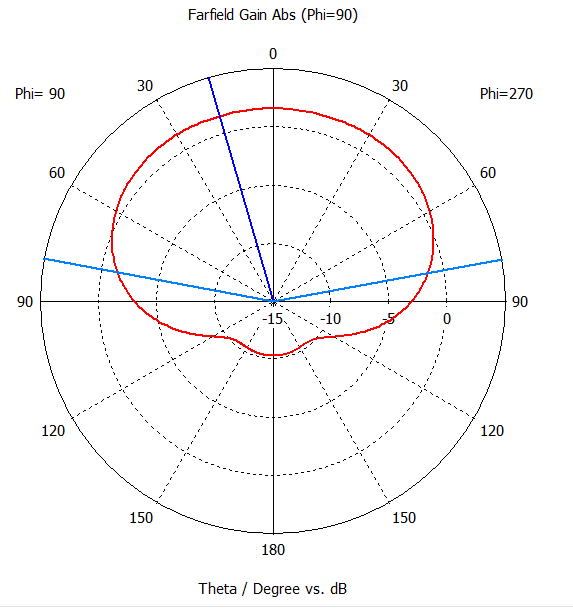
\includegraphics[scale = 0.5]{figures/antennas/qha/qha_6_ff_131}
\caption{Simulated farfield at 131MHz}
\label{fig:QHA_ff_131}
\end{figure}

\begin{figure}[H]
\centering 
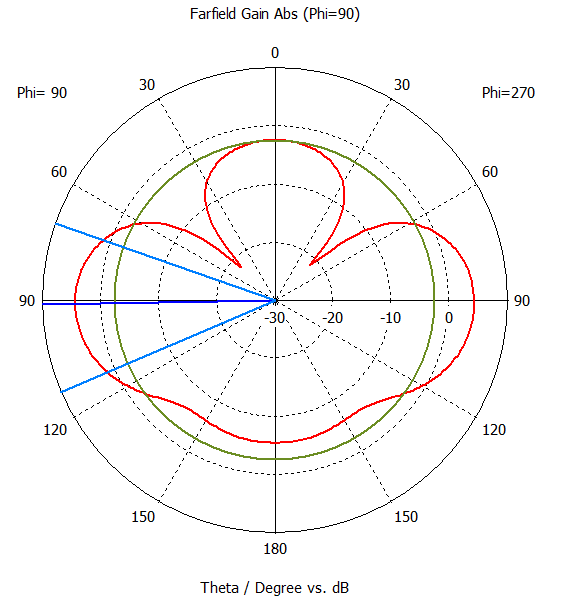
\includegraphics[scale = 0.5]{figures/antennas/qha/qha_6_ff_262}
\caption{Simulated farfield at 262MHz}
\label{fig:QHA_ff_262}
\end{figure}

\begin{figure}[H]
\centering 
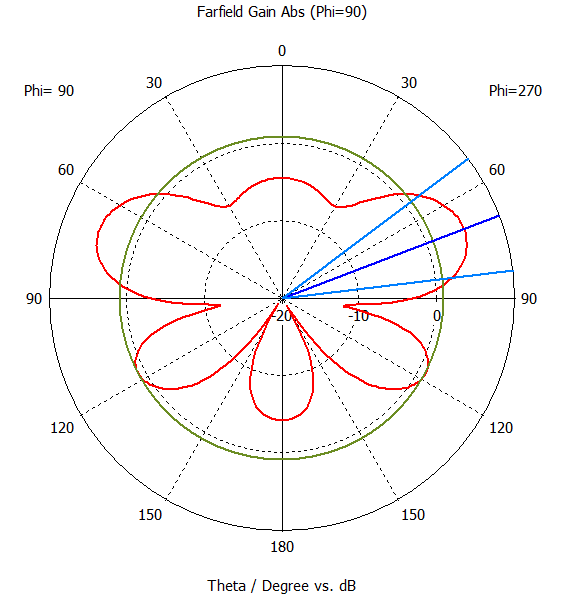
\includegraphics[scale = 0.5]{figures/antennas/qha/qha_6_ff_393}
\caption{Simulated farfield at 393MHz}
\label{fig:QHA_ff_393}
\end{figure}

%%%%%%%%%%%%%%%%%%%%%%%%%%%%%%%%%%%%%%%%%%%%%%%%%%%%%%%%%%%%%%%%%%%%%%%%%%%%%%%%%%%%% Feeding %%%%%%%%%%%%%%%%%%%%%%%%%%%%%%%%%%%%%%%%%%%%%
\subsubsection{Feeding methods}
In figure \ref{fig:QHA2} the feeding of the QHA is done using two discrete ports. When port 1 is fed with a positive phase at $90^\circ$ the QHA will have it's maximum radiation in the forward direction. If the port instead is fed with a negative phase at $90^\circ$ then the QHA will have it's maximum radiation in the backward direction. Other phases will result in non-uniform radiation patterns with one ore more peaks in the azimuth axis. It is easy to believe that it is possible to connect two of the arms of the QHA to a common ground and feed the one port with a phase difference at $90^\circ$ using a $1/4 \lambda $ transmission-line and the other directly from the source depicted in figure \ref{fig:QHA_common}. But this will not work since the geometry of the QHA will change from an electrically perspective. The shortening of the two grounds will affect the flow of the current resulting of only a pattern difference of $45^\circ$ in the farfield which then makes it impossible to archive a omnidirectional radiation pattern and circular polarization. To overcome this is has been shown in \citep{Bai2014} that it is possible to use a feeding network consisting of one second-iteration Moore $180^\circ$ hybrid coupler and two second-iteration Sierpinski $90^\circ$ hybrid couplers. It has also been showen in \citep{Yang2014} that a broadband feed network can be done using an wilkinson powerdivider and broadband $90^\circ$ phase shifters.     

\begin{figure}[H]
\centering 
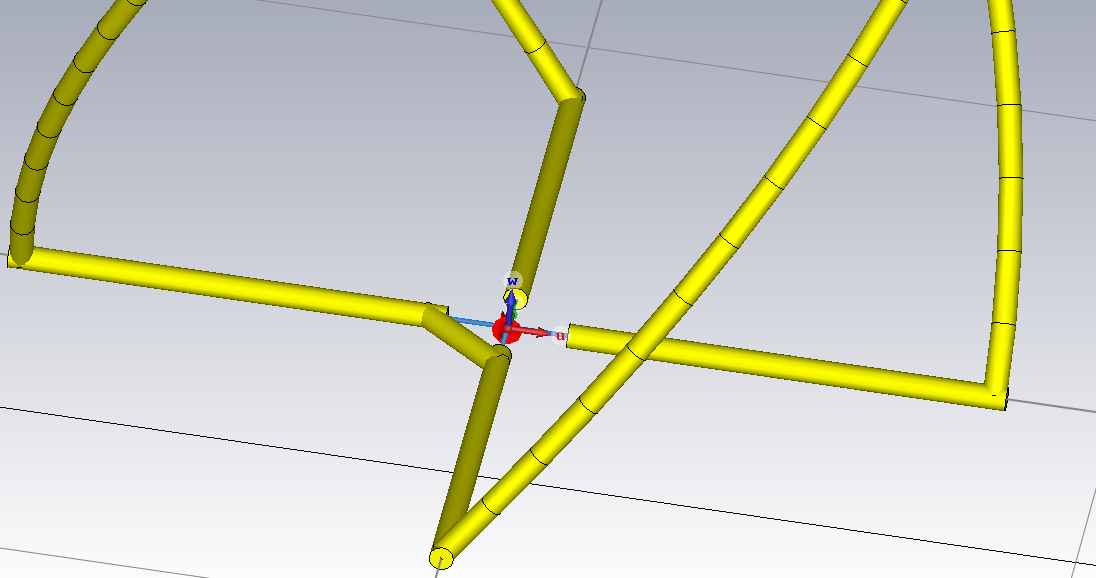
\includegraphics[scale = 0.3]{figures/antennas/qha/qha_6_common_gnd}
\caption{Common GND for the QHA}
\label{fig:QHA_common}
\end{figure}

\subsubsection{Wideband QHA}
As shown previously a QHA in its basic form radiates only at a narrow frequency band. For the S-parameters in figure \ref{fig:QHA_S11} it is seen that at 131MHz the return loss is about -2dB which results in an efficiency at only -5dB. This can be improved using a match network, but the antenna still needs to be a radiating element and therefore the matching can only improve the return-loss and not the bandwidth \citep{Iyver2010}. Therefore some modifications needs to be done at the QHA to improve the bandwith.     

%%%%%%%%%%%%%%%%%%%%%%%%%%%%%%%%%%%%%%%%%%%%%%%%%%%%%%%%%%%%%%%%%%%%%%%%%%%%%%%%%%%%%%%%%%%%%%%%%%%%%%%%%%%%%%%%%%%%%%%%%%%%%%%%%% 


\section{Spiral antennas}


\subsection{Conical Log-Spiral antenna}

\begin{figure}[H]
\centering 
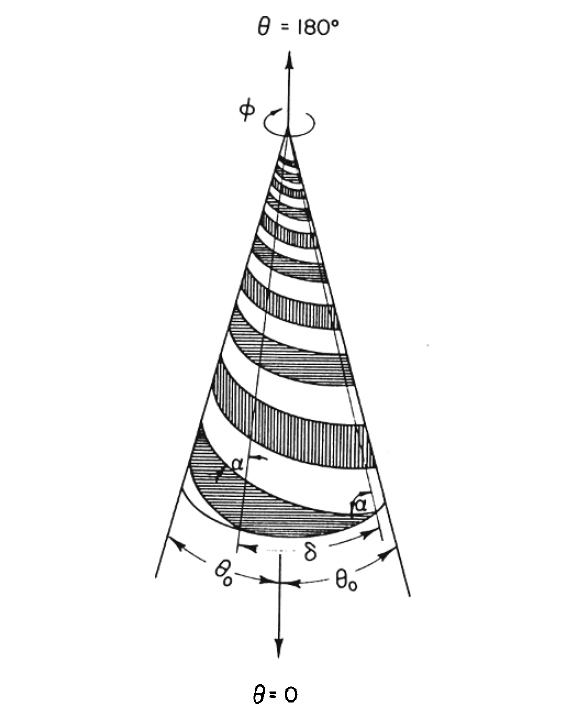
\includegraphics[scale = 0.5]{figures/antennas/spiral/conical_spiral}
\caption{Conical spiral antenna \citep{Rumsey1966}}
\label{fig:con_spi}
\end{figure}


The balanced two arm Conical Log-Spiral Antenna (CLSA) depicted in figure \ref{fig:con_spi} is a derivative of planar spiral antennas which all are frequency independent because the geometry is only described by angles \citep{Balanis2005}. The CLSA consist of two metal strips on the surface of a cone, whose shapes are defined by the equiangular spiral of equation \ref{eq:spiral} \citep{Rumsey1966}.

\begin{equation}
r = e^{\alpha\phi sin(\theta_0)}
\end{equation}
\label{eq:spiral} 

The angle $\alpha$ between the radius and the tangent to the spiral is $cot^{-1}(\alpha)$ and because of the spiral $\theta_0 = 90^\circ$. The CSA do also have circular polarization which makes it usable for satellite communication. 



%%%%%%%%%%%%%%%%%%%%%%%%%%%%%%%%%%%%%%%%%%%%%%%%%%%%%%%%%%%%%%%%%%%%%%%%%%%%%%%%%%%%%%%%%%%%%%%%%%%%%%%%%%%%%%%%%%%%%%%%%%%%%%

\section{Horn antennas}
\section{Printed antennas}










    



   